\documentclass{standalone} 
\usepackage{tikz}
\usetikzlibrary{arrows,positioning,automata,shadows,fit,shapes}
\tikzstyle{block} = [rectangle, draw, fill=blue!20, 
    text width=6em, text centered, rounded corners, minimum height=4em]
    \tikzstyle{line} = [draw, -latex']
\begin{document}
    \begin{tikzpicture}[line,>=stealth]
        \node [color=gray] (1) { 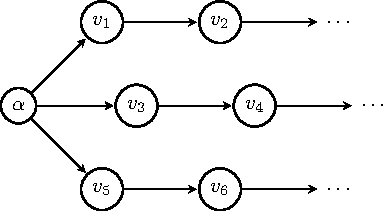
\includegraphics[scale=0.7]{realSystem.pdf}};
        \node[above= 0cm of 1]{Real system};
        \node [color=blue,right = of 1] (2) {$\alpha\to\cdots\to \omega?$ };
        \node [below = of 1] (3) {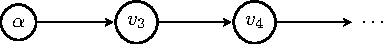
\includegraphics[scale=0.7]{partialObservation.pdf}};
        \node[below= 0cm of 3]{Partial observation};
        \node [right = of 3] (4) {Learning approaches};
        \node [right = of 4] (8) {Model};
        \draw [->] (4) -- (8);
        \node [color=blue,right = of 8] (5) {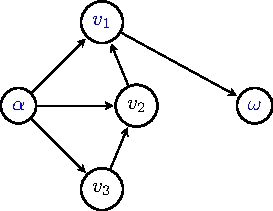
\includegraphics[scale=0.7]{reachability.pdf}};
        \node[above= -0.2cm of 5]{Reachability};
        \node [color = red, below left = 2cm and -1.5cm of 5] (7) {Model Checking};
        \node [color=blue,above = of 2] (6) {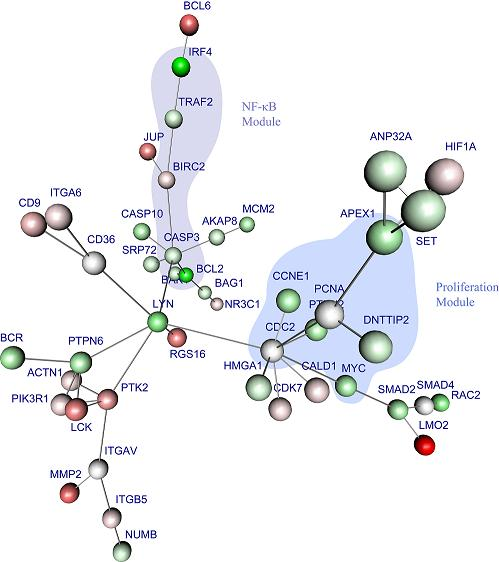
\includegraphics[scale=0.3]{biologicalNetwork.jpg}};
        \node [right = -0.2cm of 6] {Biological \textit{a priori} knowledge};
        \draw [dashed,->] (1) -- (6);
        \draw [color=blue,->] (2) -- (5);
        \draw [dashed,->] (1) -- (3);
        \draw [->] (3) -- (4);
        %\draw [->] (8) -- (5);
        \draw [color=blue, ->] (6) -- (2);
        \node [below = of 5] (9) {$+$};
        \draw [->] (8) --(9);
        \draw [->] (5) --(9);
        \draw [->] (9) --(7);
        \draw[thick, color=red] (7)--(8);
    \end{tikzpicture}
\end{document}